\documentclass{article}
\usepackage[margin=1in]{geometry}
\usepackage{tabulary}
\usepackage{float}
\usepackage{lipsum}
\usepackage[utf8]{inputenc}
\usepackage{hyperref}
\usepackage{graphicx}
\usepackage{graphics}

\begin{document}
\begin{center}{\LARGE ECE 264: Advanced C Programming} \end{center}
\begin{center}{\large Lecture Notes 6/10/19} \end{center}

\bigskip

\section{Topics}
\begin{enumerate}
\item GitHub (live demo)
	\begin{enumerate}
	\item Initializing a repository: cloning a git repo
	  \begin{enumerate}
	    \item Using HTTPS on ECN machines
	    \item Using SSH (including generating SSH keypair)
	  \end{enumerate}
	\item Adding content: how to add and commit
	\item Saving content on remote: how to push
	\item Making releases: how to tag
	\end{enumerate}
\item Makefiles
  \begin{enumerate}
  \item Format
  \item Macros
  \end{enumerate}
\item Selection sort (brief introduction)
\end{enumerate}


\section{Version Control}
This class uses Git for version control. Git is a distributed version control system. That means there are two repositories: local and remote. When you commit changes, only the local repository is changed. This makes commits fast and independent of network connections. If your computer is damaged, you still lose the local repository. To change the remote repository, you need to push the changes. If your computer is damaged, you can retrieve the code from the remote repository. Please push your code to GitHub often. Not only does that prevent you from losing any code if you accidentally delete anything, it helps us help you debug, by giving us access to your latest code.

Please read the book about how to use version control: https://git-scm.com/book/en/v2

We did a live demo showing the following steps:
\begin{enumerate}
\item Show HTTPS clone on ecegrid machine
\item Show SSH setup and clone on ecegrid machine
\item Show git status, git add, git commit, git push
\item Show git tag
\end{enumerate}

\paragraph{Setting up a GitHub Account} create a Github account (if you do not already have one). This is the account you should use to create and submit all of your assignments this semester.
Also let us know your account name by filling in the Google Form provided in BlackBoard and Piazza.

\paragraph{Setting up SSH key with GitHub}
Set up a public SSH key in your GitHub account (if you haven't already). To do this, first generate a new ssh key:

\texttt{> ssh-keygen} \linebreak
Hit enter three times (to accept the default location, then to set and confirm an empty passphrase). This will create two files: ~/.ssh/id\_rsa (your private key) and ~/.ssh/id\_rsa.pub (your public key)
Then print out your public key:

\texttt{> cat ~/.ssh/id\_rsa.pub} \linebreak
And copy it to the clipboard. 
Then follow steps at: \href{https://help.github.com/en/articles/adding-a-new-ssh-key-to-your-github-account}{https://help.github.com/en/articles/adding-a-new-ssh-key-to-your-github-account} 

\section{Makefile}
Makefiles let you define complicated sets of commands to build your projects.

\begin{flushleft}Makefiles consist of a series of rules:\end{flusheft} \linebreak
\texttt{[target] : [dependences]} \linebreak
\texttt{[TAB] \quad command 1}\linebreak
\texttt{[TAB] \quad command 2}\linebreak
\texttt{...}
%[TAB] \quad command 2\linebreak
%...}

A rule \emph{target} is the name of the rule. The \emph{dependences} are the files the rule depends on. The \emph{commands} are what to do when the rule is ``fired''. Note: there must be a tab before each command.

A rule is fired in one of two ways: (i) it is directly invoked (by calling ``make [target]'') or (ii) it is invoked by another rule that is fired. 

When a rule is fired, it goes through the following process:
\begin{enumerate}
\item If a \emph{dependence} has a rule in the Makefile, fire that rule (using this same process)
\item Once all dependences have been fired, check to see if \emph{target} is ``out of date'': interpret \emph{target} as a filename, and see if the timestamp on the file is older than the time stamp on any of its dependences. 
If it is, the target is ``out of date''. If there is no file named \emph{target}, the target is always assumed to be out of date. If there are no dependences and \emph{target} exists, target is assumed to be up to date.
\item If the target is out of date, execute the list of commands 
\end{enumerate}

You can use Makefiles to orchestrate complicated build processes.\linebreak
If you type ``make'' without a target, make will fire the first rule in the Makefile. \linebreak
We usually define a target called ``clean'' whose job it is to clean up any intermediate files
generated during the build process. This can also be used to remove all generated targets to
force recompiling everything. \linebreak

\begin{flushleft}
Makefiles also let you define macros to reuse the same commands over and over. For example,
we can define GCC as a macro that invokes gcc the way we want:\end{flushleft}
\linebreak
\linebreak
\texttt{DEBUG = -DDEBUG \linebreak
CFLAGS = CFLAGS = -std=c99 -g -Wall -Wshadow --pedantic -Wvla -Werror \linebreak
GCC = gcc \$(CFLAGS) \$(DEBUG) } 
\linebreak
\linebreak
Note that we use \$(MACRO\_NAME) to insert the macro into other places, including commands.
Makefiles can get much more complicated than this, but their full power is beyond the scope of
this course.


\section{Selection Sort}
\paragraph{Readings:} Forouzan and Gilberg, pp 491-493

Selection sort is one particular sorting algorithm that sorts an array using the following procedure: Divide the array up into two pieces (we'll call them ``sorted'' and ``rest''). \emph{Sorted} is the portion of
the array that is already sorted. \emph{Rest} is the rest of the array. One thing that is always true (an invariant) is that all the elements in \emph{sorted} are smaller than any of the elements in \emph{rest}.
Selection sort works by slowly growing the sorted side of the array and shrinking the rest of the array. Think of this as having a cursor. When the sorting starts, we don't know if any of the array 
is sorted, so our cursor starts out pointing to the first element of the array. Everything to the left of the cursor (colored green, in this case nothing!) is sorted:

\begin{figure}[H]
\centering
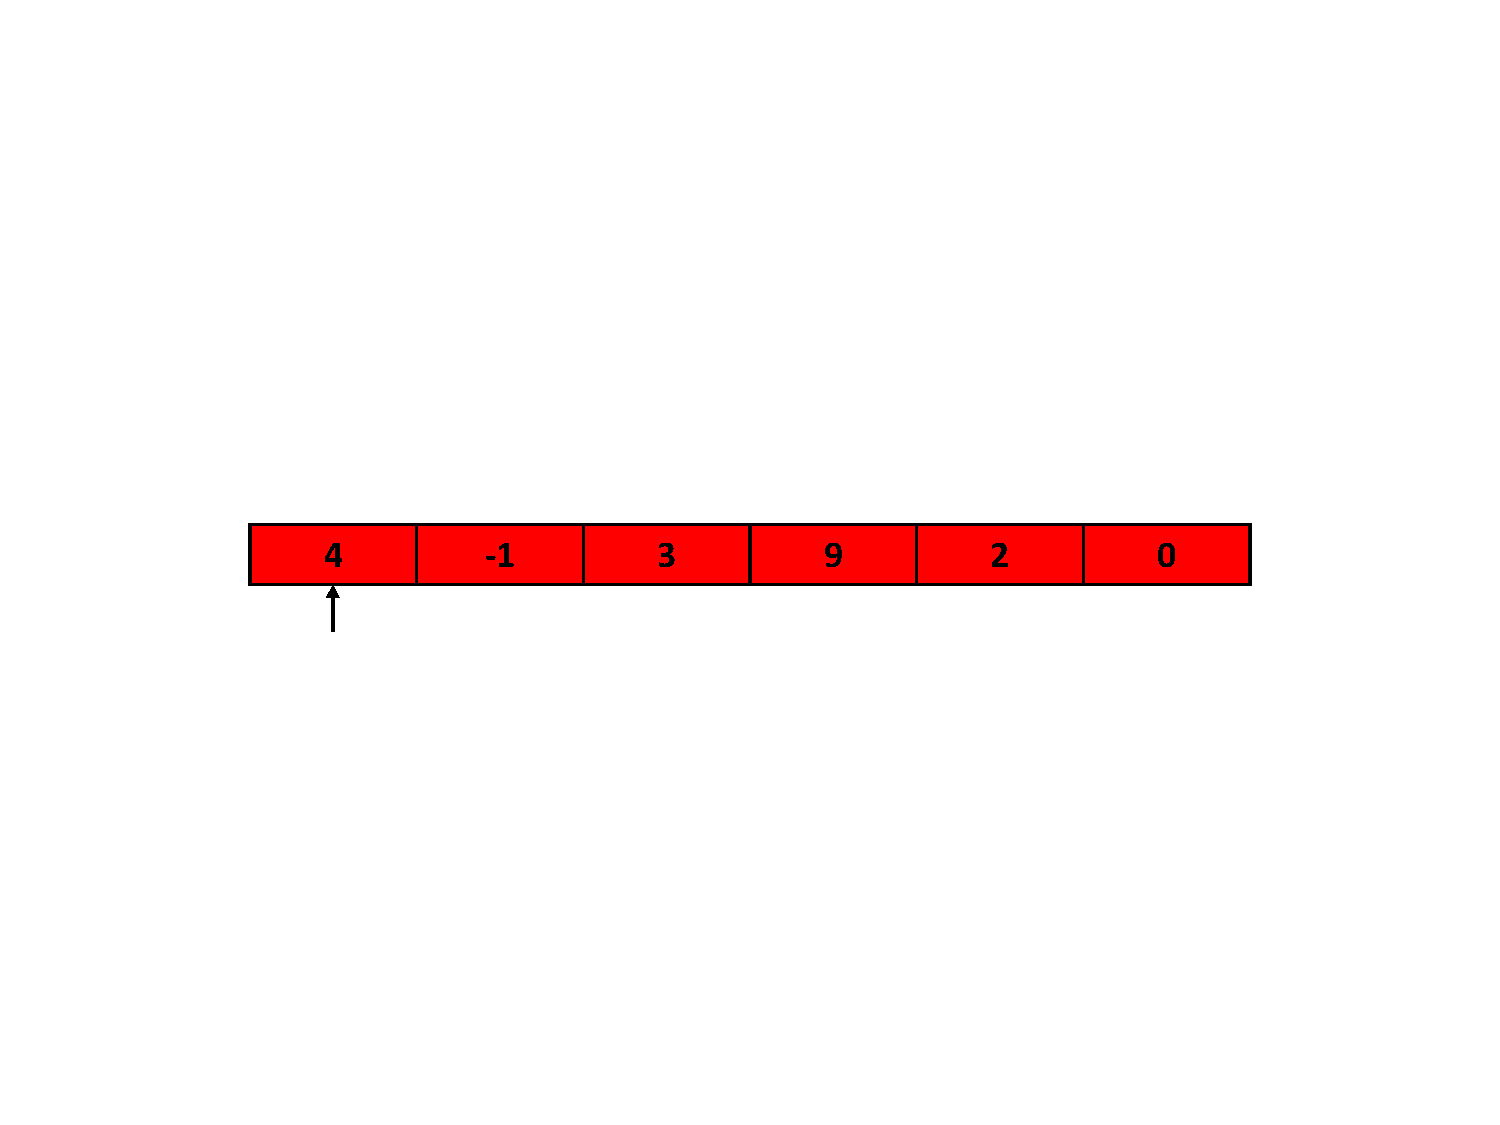
\includegraphics[scale=0.5]{Fig1}
\end{figure}

Everything from the cursor to the right (colored red) is the rest of the array. We then scan
through the rest of the array to find the smallest element, and swap it with the element at the
cursor (this might be the element itself!):

\begin{figure}[H]
\centering
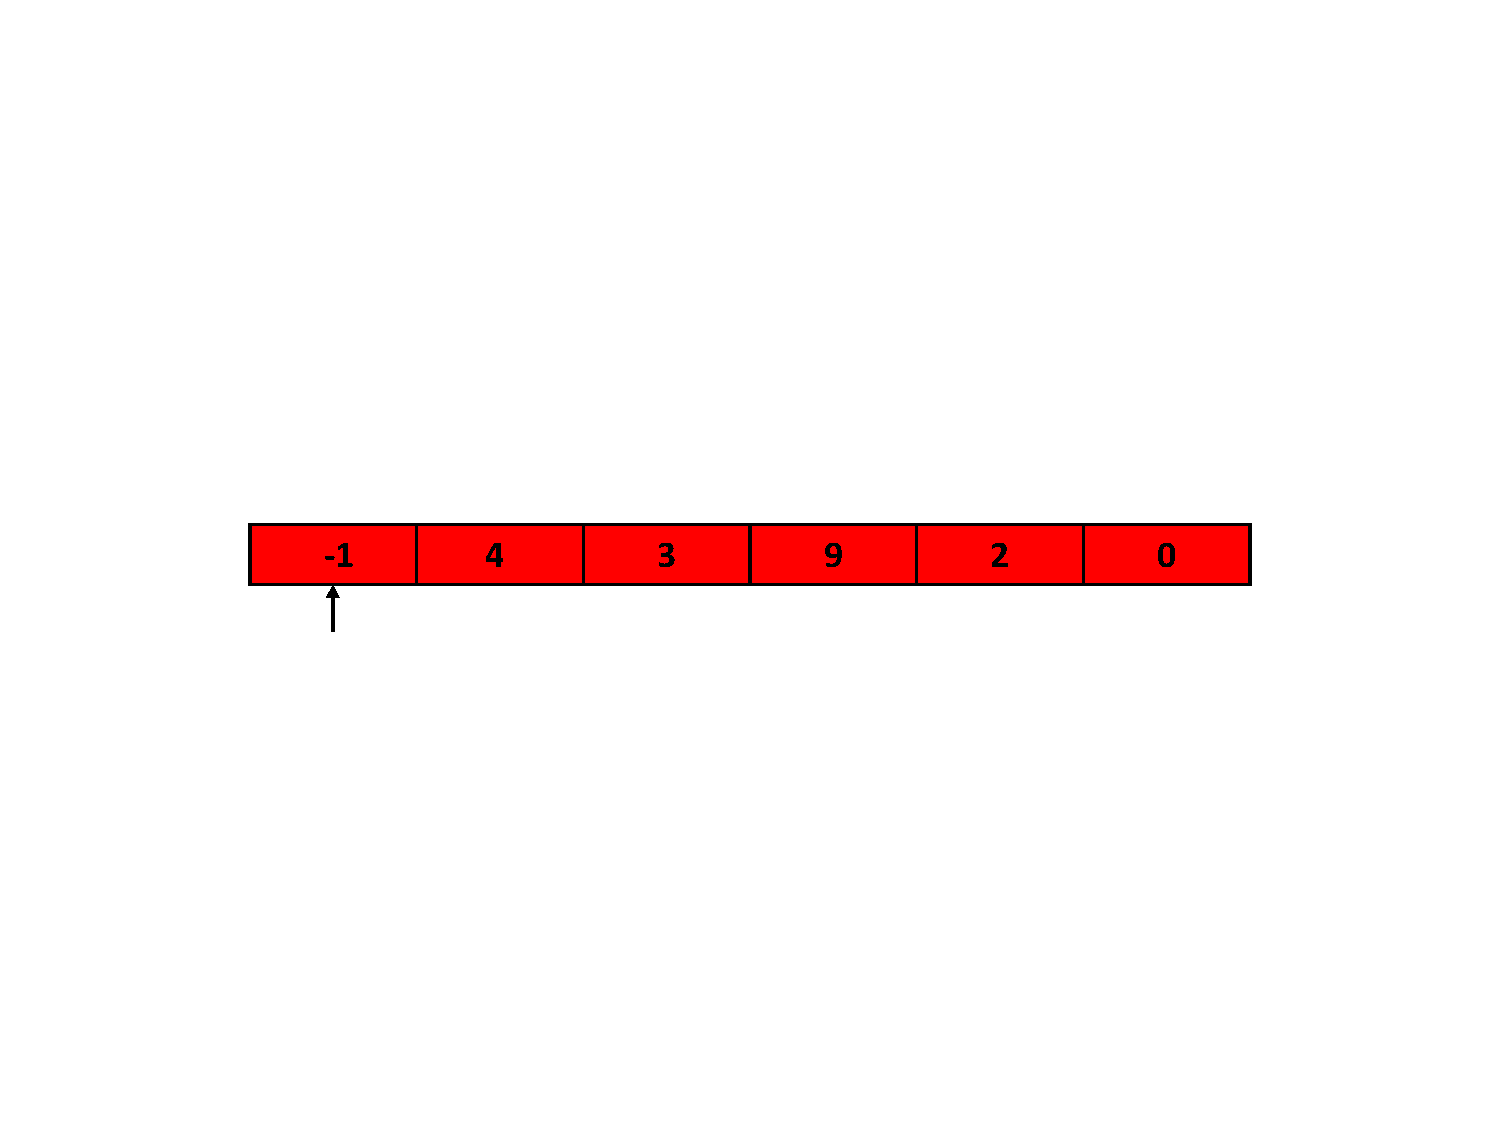
\includegraphics[scale=0.5]{Fig1_1}
\end{figure}

Because we just moved the smallest element to the cursor, we can now move the cursor up
one:

\begin{figure}[H]
\centering
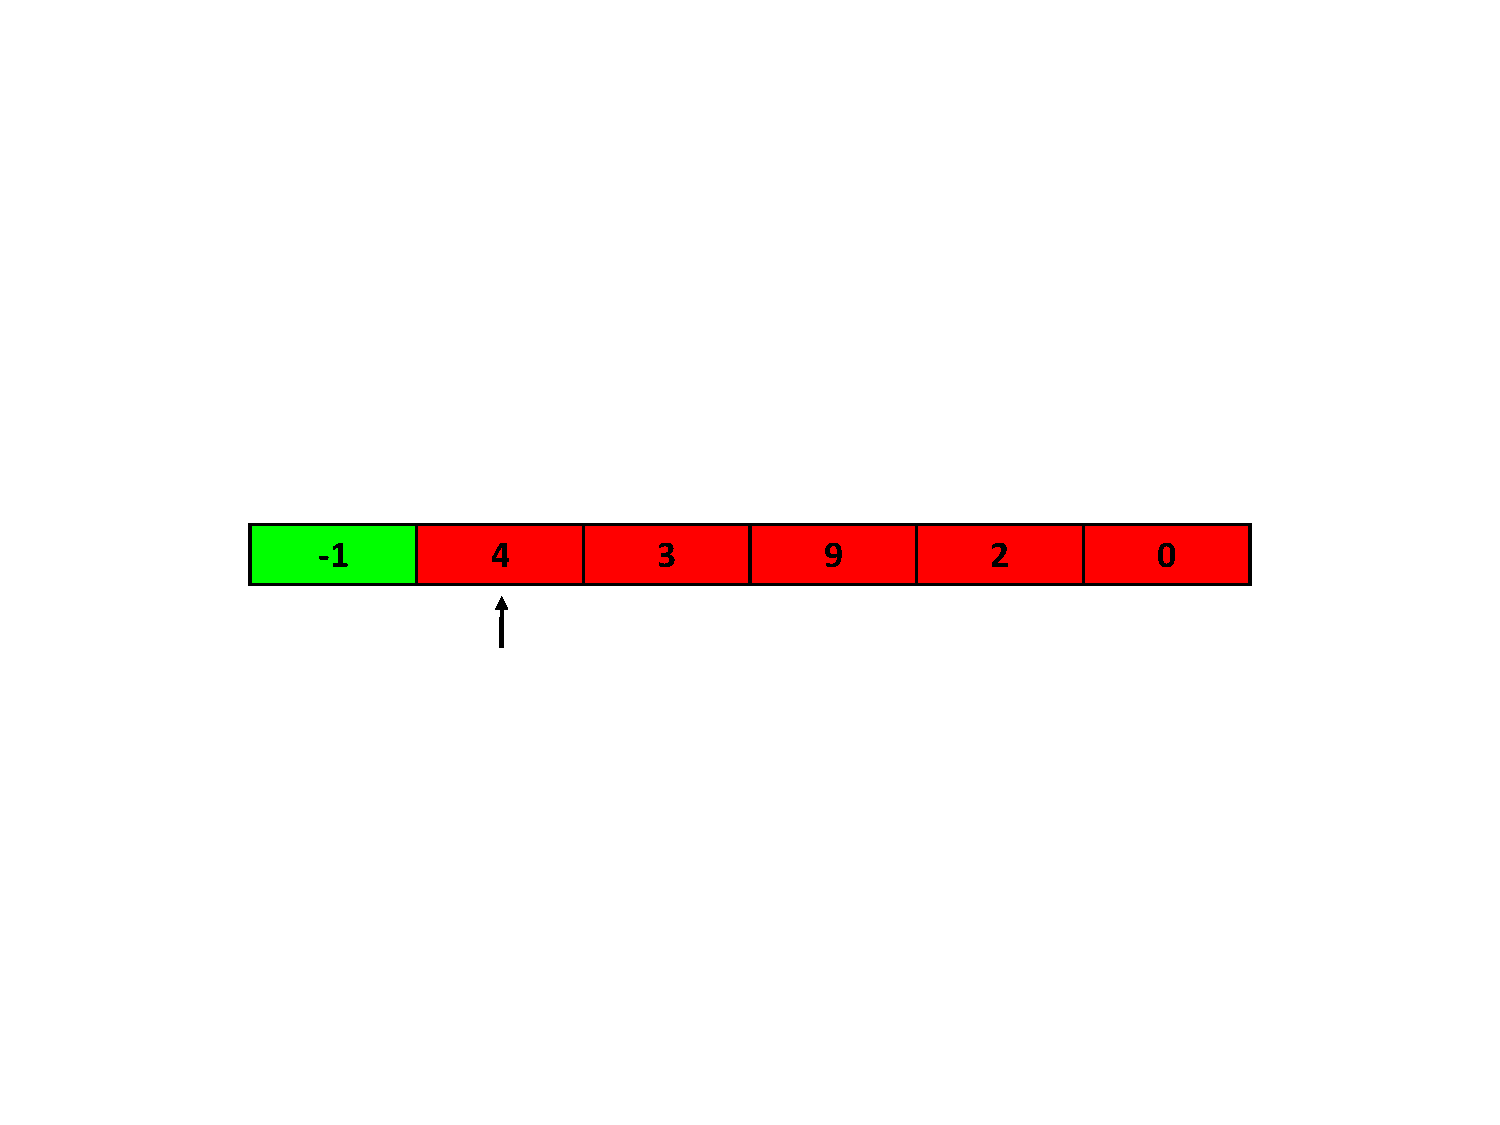
\includegraphics[scale=0.5]{Fig2}
\end{figure}

Note that our rules still hold: everything to the left of the cursor is sorted, and everything from
the cursor right is larger than anything in the sorted part of the array. Now we repeat the
process, finding the smallest element in the rest of the array and swapping it with the cursor:

\begin{figure}[H]
\centering
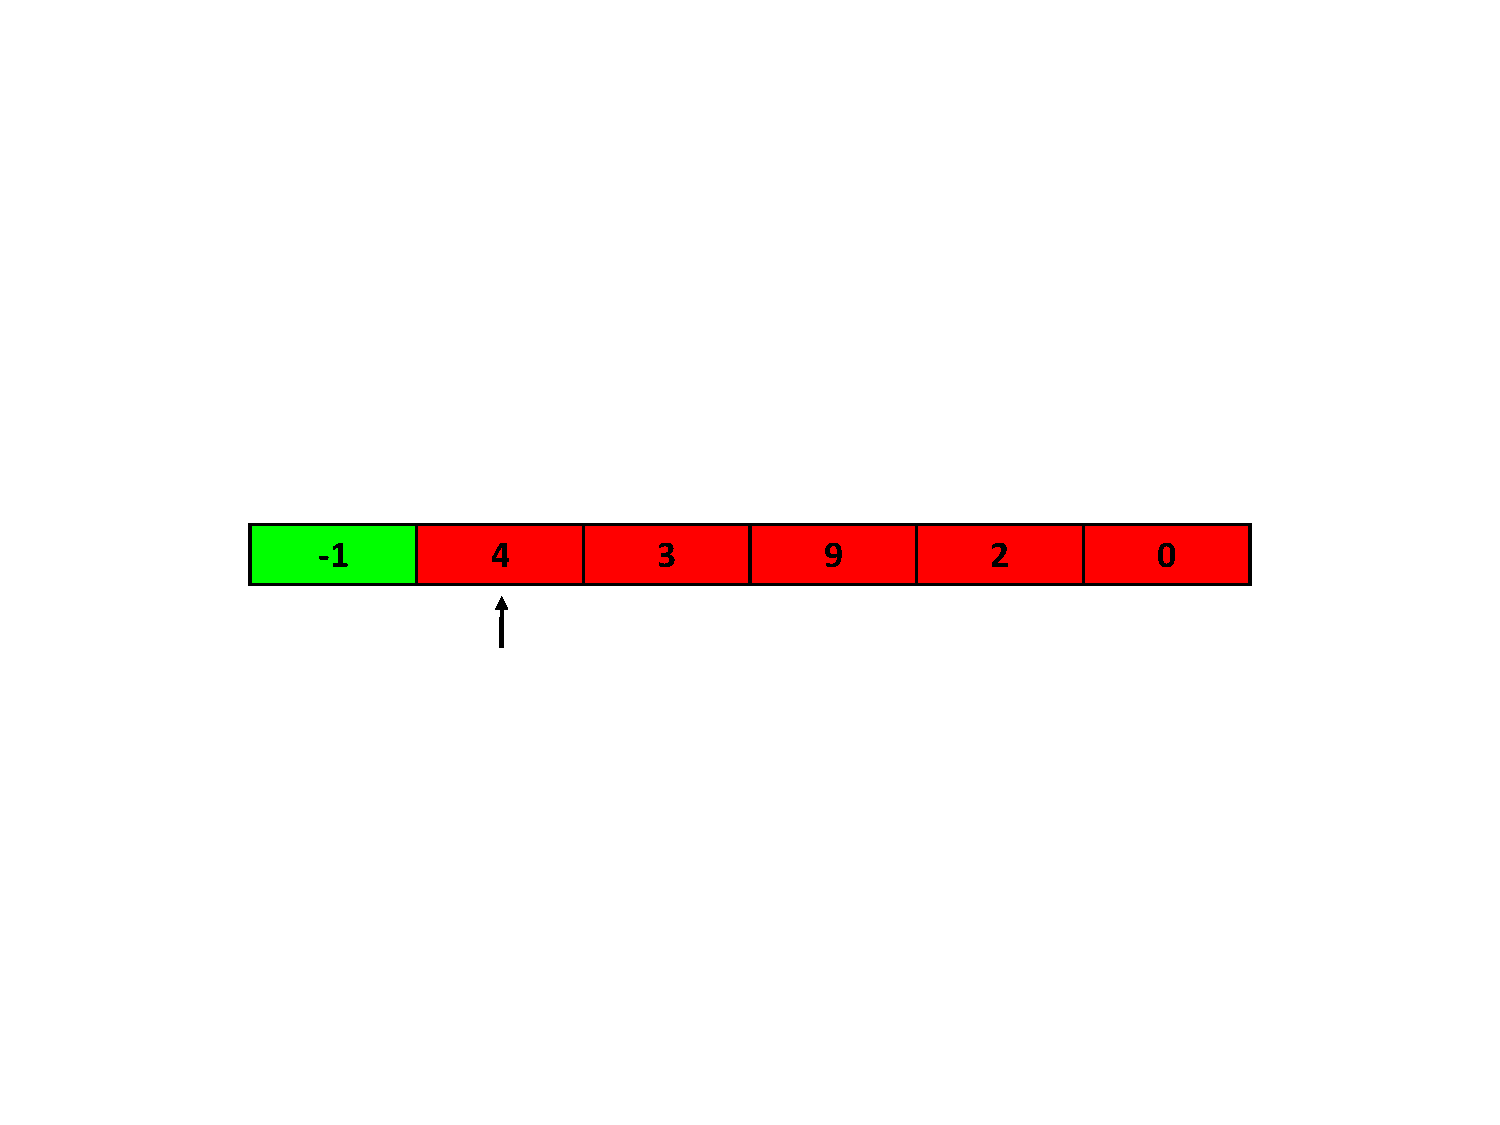
\includegraphics[scale=0.5]{Fig2}
\end{figure}

And we can now move the cursor to the right again, restoring our properties. The sorted part of
the list is sorted, and the rest of the list is larger than anything in the sorted part of the list:

\begin{figure}[H]
\centering
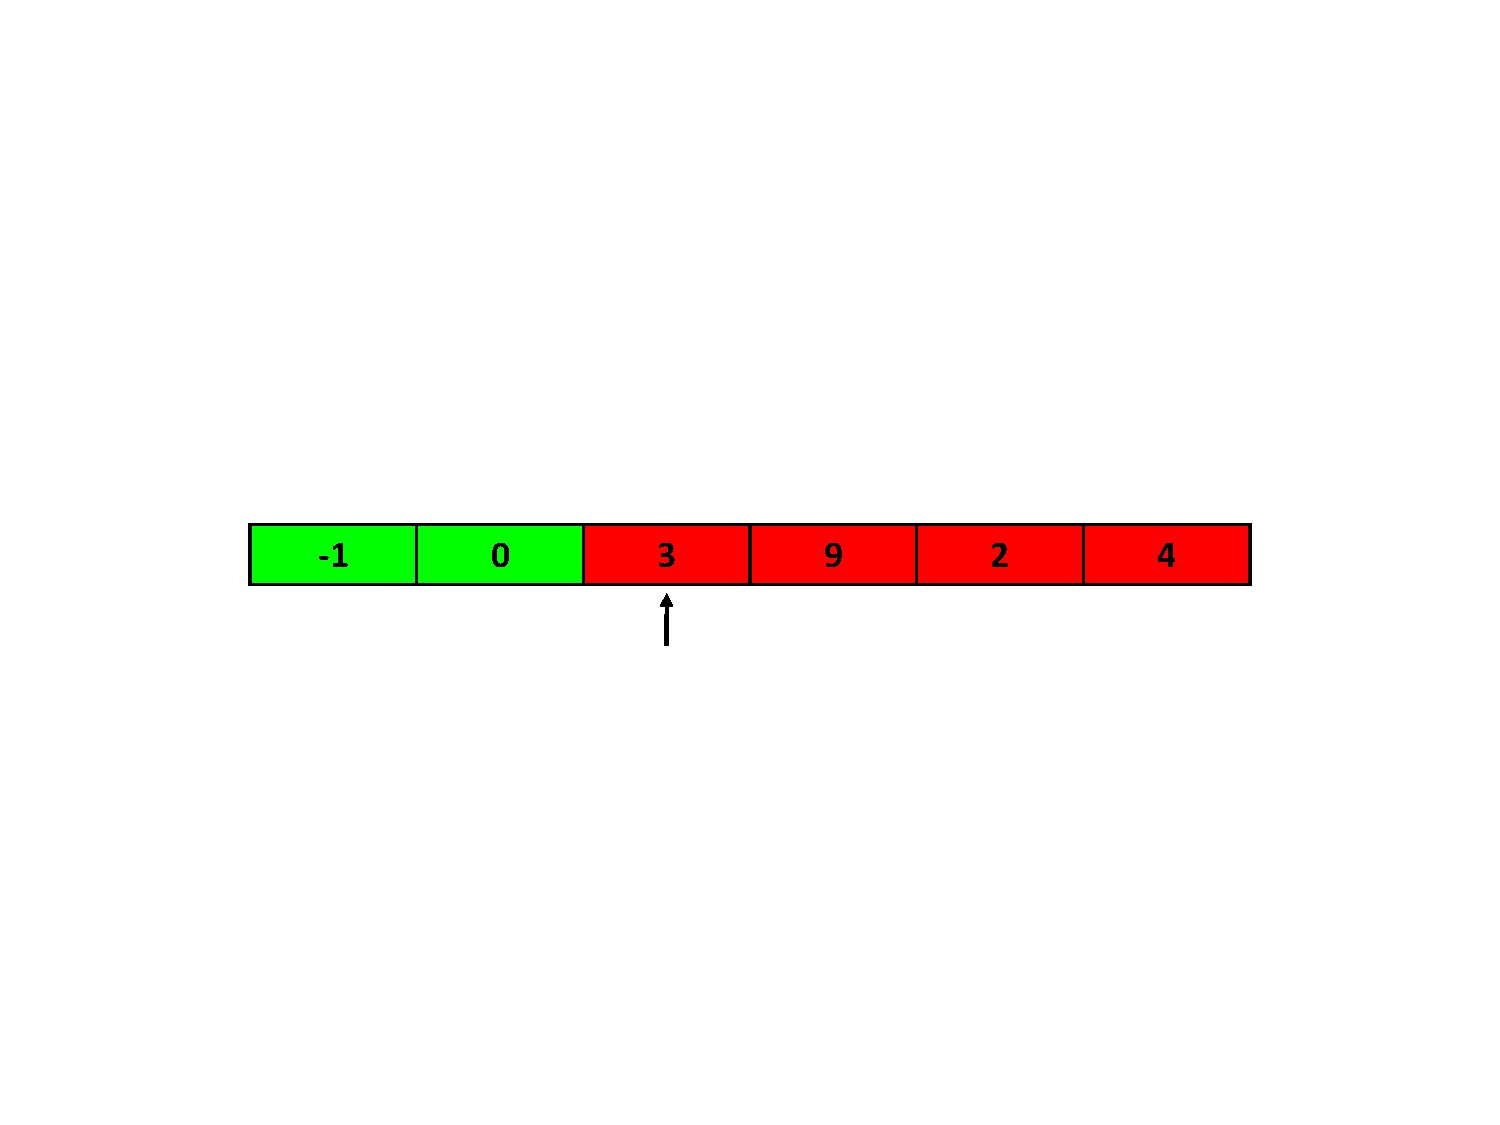
\includegraphics[scale=0.5]{Fig3}
\end{figure}

Note that each time we repeat this process, the cursor moves one to the right. The sorted list
gets longer, and the rest of the list gets shorter. In this manner, we eventually sort the list:

\begin{figure}[H]
\centering
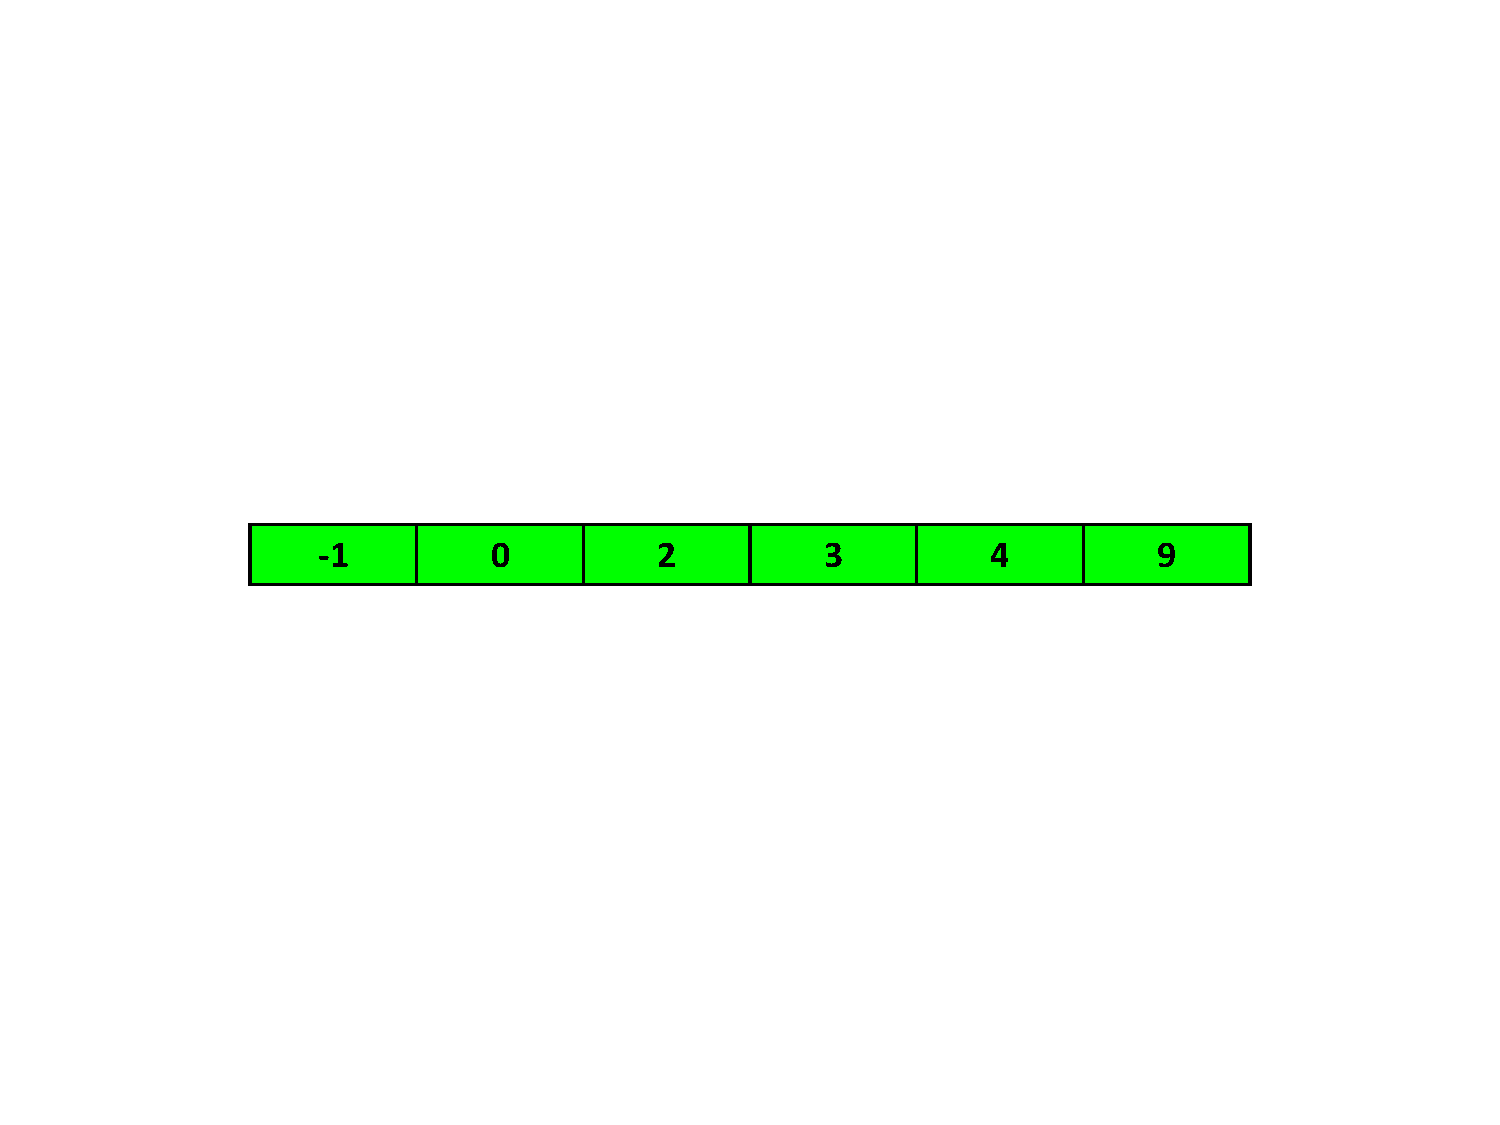
\includegraphics[scale=0.5]{Fig4}
\end{figure}

We will use pseudocode for most of our code examples in class. This lets us quickly explain the
structure of an algorithm without worrying about nitty-gritty details of correct C syntax. It also
means that we can describe an algorithm without giving you code that you can just copy for an
assignment!
\end{document}
